Facciamo ora un riassunto delle forze coinvolte nei processi di dissoluzione.

Le forze intermolecolari sono attrazioni intermolecolari che si esercitano tra atomi, molecole o ioni. Parleremo di ioni quando avremo a che fare con elettroliti, mentre parleremo di molecole quando avremo soluzioni di non elettroliti, ad esempio acqua e saccarosio. Infine parleremo di atomi quando avremo a che fare con soluzioni di speci atomiche.
\subsection{Forze ione-ione}
Sono le interazioni più forti. Si esercitano tra ioni di carica opposta e tale forza è la forza di Coulomb:

\begin{minipage}{0.5 \textwidth}
    \vspace{1cm}
    $$F \propto \frac{q_1 \cdot q_2}{d^2}$$
\end{minipage}
\begin{minipage}{0.5 \textwidth}
    \begin{figure}[H]
        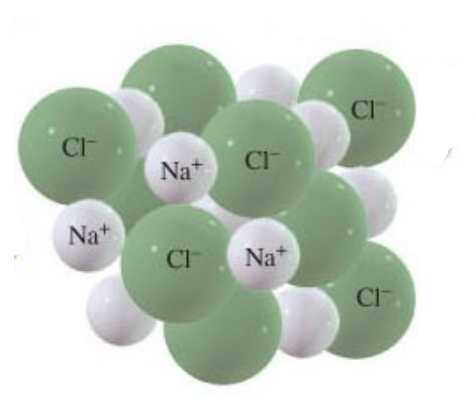
\includegraphics[width=4cm]{immagini/forze_ione_ione.png}
    \end{figure}
\end{minipage}

\subsection{Forze ione-dipolo}
L'acqua è una molecola dipolare, cioè ha un forte momento di dipolo. Pertanto sono queste le forze in gioco nei processi di dissoluzione degli elettroliti o di solidi ionici. La forza cioè sarà proporzionale al prodotto della carica del singolo ione per il momento di dipolo della molecola in questione, come ad esempio l'acqua:

\begin{minipage}{0.5 \textwidth}
    \vspace{0.2cm}
    $$F \propto \frac{q \cdot \mu}{d^2}$$
\end{minipage}
\begin{minipage}{0.5 \textwidth}
    \begin{figure}[H]
        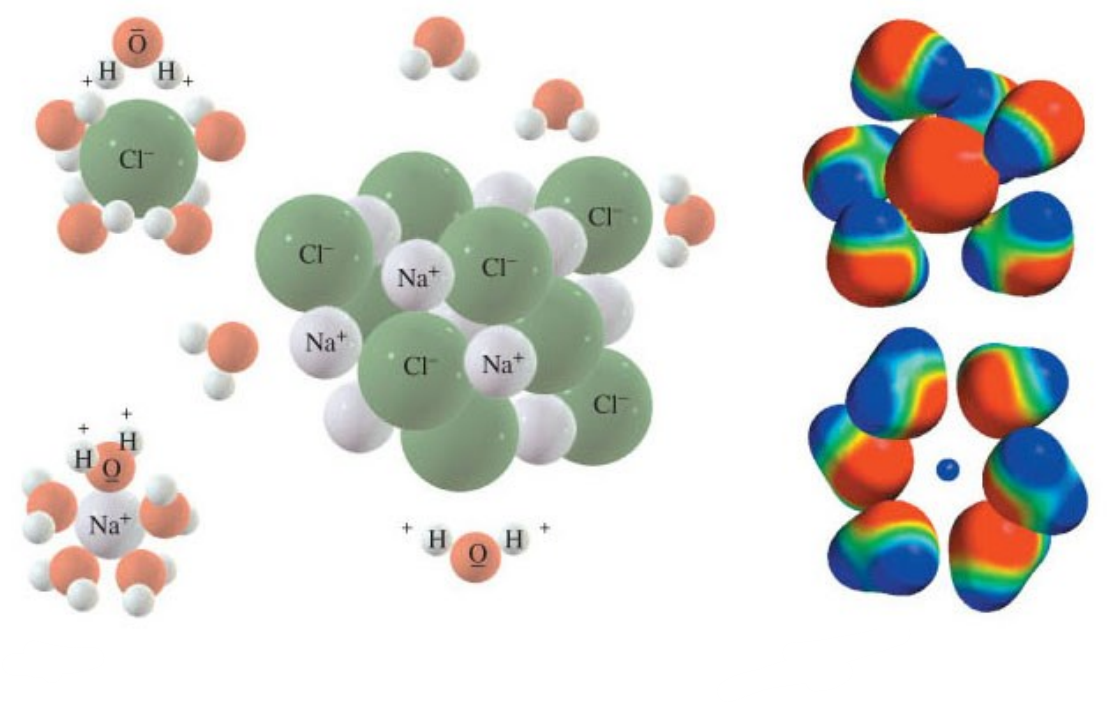
\includegraphics[width=7cm]{immagini/forze_ione_dipolo.png}
    \end{figure}
\end{minipage}

\subsection{Forze dipolo-dipolo}
Abbiamo visto il legame ad idrogeno. Più in generale le forze che si esercitano tra molecole che possiedono momenti di dipolo permanenti sono forze date dal prodotto dei momenti di dipolo diviso la distanza al cubo:

$$F \propto \frac{\mu_1 \cdot \mu_2}{d^3}$$

Tali forze si hanno sia se le molecole dotate di momento di dipolo sono uguali sia se sono diverse, come nel caso di acqua e metanolo CH$_3$OH. In questo caso l'idrogeno legato all'ossigeno del metanolo interagisce con l'ossigeno di una molecola d'acqua. Non interagiscono gli altri tre perché il legame carbonio-ossigeno è poco polare a differenza di quello carbonio-ossigeno. Infatti la carica di questo legame è fortemente spostata verso l'ossigeno, quindi l'idrogeno ha una forte carica positiva e può interagire con l'ossigeno di una molecola d'acqua.

\hspace{0.5cm}\begin{minipage}{0.35 \textwidth}
    \begin{figure}[H]
        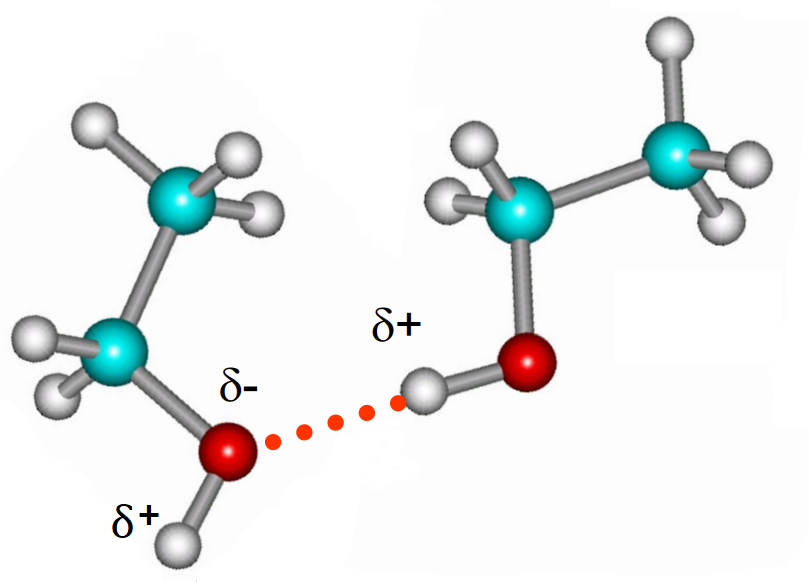
\includegraphics[width=5cm]{immagini/alcol_etilico.png}
    \end{figure}
\end{minipage}
\begin{minipage}{0.6 \textwidth}
    \vspace{0.6cm}Un altro esempio sono due molecole di alcol etilico CH$_3$CH$_2$OH. Anche qui i legami non carbonio-idrogeno sono fortemente polari, mentre il legame ossigeno-idrogeno lo è. Ecco quindi che l'idrogeno del gruppo OH di una molecola interagirà con l'ossigeno del gruppo OH dell'altra molecola, facendo instaurare una interazione.
\end{minipage}

\hspace{0.5cm}\begin{minipage}{0.35 \textwidth}
    \begin{figure}[H]
        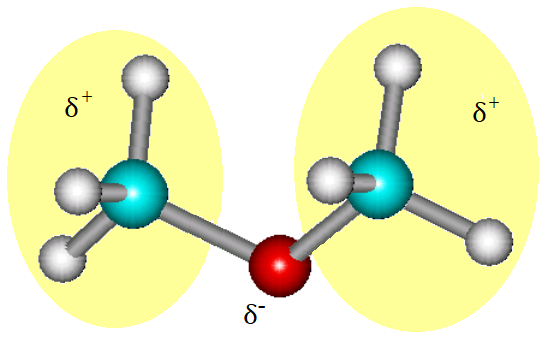
\includegraphics[width=5cm]{immagini/etere_dimetilico.png}
    \end{figure}
\end{minipage}
\begin{minipage}{0.6 \textwidth}
    \vspace{0.6cm}Anche l'etere dimetilico può dare luogo a legami polari che possono essere coinvolti in ulteriori interazioni ad idrogeno. L'etere dimetilico ha formula CH$_3$OCH$_3$ e in esso l'ossigeno ha una parziale carica negativa perché i gruppi CH$_3$ risultano positivizzati dall'elettronegatività dell'ossigeno che porta questo ad attirare su di sé cariche elettroniche che sottrae a tali gruppi. In questa molecola il momento di dipolo è ancora più basso perché fondamentalmente abbiamo interazioni carbonio-ossigeno.
\end{minipage}

\vspace{0.2cm}Va da ricordare che i legami a idrogeno sono inoltre responsabili dell'alto punto di ebollizione di alcune speci.

\hspace{0.5cm}\begin{minipage}{0.35 \textwidth}
    \begin{figure}[H]
        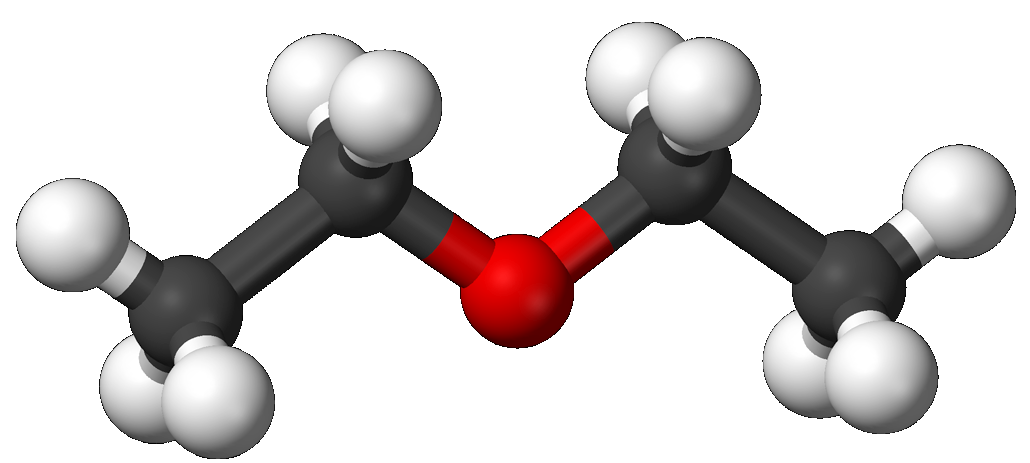
\includegraphics[width=5cm]{immagini/etere_dietilico.png}
    \end{figure}
\end{minipage}
\begin{minipage}{0.6 \textwidth}
    \vspace{0.6cm}Se infine consideriamo l'etere dietilico C$_2$H$_5$OC$_2$H$_5$, questa molecola ha un momento maggiore e un punto di fusione maggiore di quelli dell'etere dimetilico. Ciò avviene perché i legami a idrogeno non sono l'unica interazione debole che determina momenti di dipolo e punti di ebollizione. Nel caso particolare, fra le catene laterali possono esercitarsi alcuni tipi di interazioni dette di \textit{Van der Waals}.
\end{minipage}

\vspace{0.2cm}Quindi tutte quelle volte che vogliamo portare ad esempio ad ebollizione un dato composto, certamente la massa del composto ha un ruolo, ma le interazioni da rompere fra le singole molecole (A-A se è una specie chimica, A-B se è una soluzione di A e B) possono essere determinanti, qualora si instaurino.

\subsection{Forze ione-dipolo indotto o dipolo-dipolo indotto}
Alcune molecole non hanno momento di dipolo permanente, ma in esse si può generare un momento di dipolo indotto quando ad esse avviciniamo qualcosa di carico.

Sia avvicinare uno ione che un momento di dipolo ad una molecola che non abbia un momento di dipolo permanente fa si che si generi un momento di dipolo indotto. Quello che succede è che la nube elettronica viene distorta, generando una separazione di cariche.

Sotto forma di simboli avremo

\begin{figure}[htp]
    \centering
    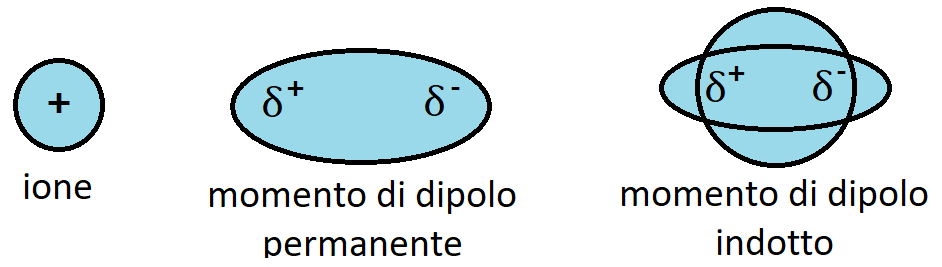
\includegraphics[width=11cm]{immagini/ioni_e_momenti_di_dipolo.png}
\end{figure}

Ci sono infine anche delle \textbf{forze dipolo indotto-dipolo indotto} che prendono il nome di \textit{Forze di London o di dispersione}

In tutto questi casi le forze esercitate hanno l'andamento di $1/d^6$
\subsection{La viscosità}
Le ultime due classi di forze sono quelle che determina la viscosità di un liquido, la quale non è altro che il suo attrito interno (Attenzione! \E diversa dalla densità).

Va da ricordare che le interazioni ad idrogeno vengono rotte facilmente, infatti se riscaldiamo esse vengono meno, insieme alle interazioni di Van der Waals. Se vengono meno ne segue che la viscosità di un liquido diminuisce all'aumentare della temperatura.